% !TEX encoding = UTF-8 Unicode

% This is a simple template for a LaTeX document using the "article" class.
% See "book", "report", "letter" for other types of document.

\documentclass[11pt]{article} % use larger type; default would be 10pt

\usepackage[utf8]{inputenc} % set input encoding (not needed with XeLaTeX)

%%%% Examples of Article customizations
% These packages are optional, depending whether you want the features they provide.
% See the LaTeX Companion or other references for full information.

%%% PAGE DIMENSIONS
\usepackage{geometry} % to change the page dimensions
\geometry{a4paper} % or letterpaper (US) or a5paper or....
% \geometry{margin=2in} % for example, change the margins to 2 inches all round
% \geometry{landscape} % set up the page for landscape
%   read geometry.pdf for detailed page layout information

\usepackage{graphicx} % support the \includegraphics command and options

% \usepackage[parfill]{parskip} % Activate to begin paragraphs with an empty line rather than an indent

\usepackage{float}
\restylefloat{table}

%%% PACKAGES
%\usepackage{booktabs} % for much better looking tables
%\usepackage{array} % for better arrays (eg matrices) in maths
%\usepackage{verbatim} % adds environment for commenting out blocks of text & for better verbatim
\usepackage{subfig} % make it possible to include more than one captioned figure/table in a single float
% These packages are all incorporated in the memoir class to one degree or another...


%%% HEADERS & FOOTERS
\usepackage{fancyhdr} % This should be set AFTER setting up the page geometry
\pagestyle{fancy} % options: empty , plain , fancy
\renewcommand{\headrulewidth}{0pt} % customise the layout...

%%% SECTION TITLE APPEARANCE
%\usepackage{sectsty}
%\allsectionsfont{\sffamily\mdseries\upshape} % (See the fntguide.pdf for font help)
% (This matches ConTeXt defaults)

%%% ToC (table of contents) APPEARANCE
%\usepackage[nottoc,notlof,notlot]{tocbibind} % Put the bibliography in the ToC
%\usepackage[titles,subfigure]{tocloft} % Alter the style of the Table of Contents
%\renewcommand{\cftsecfont}{\rmfamily\mdseries\upshape}
%\renewcommand{\cftsecpagefont}{\rmfamily\mdseries\upshape} % No bold!

%%%Include also .svg graphics
\usepackage{svg}

%%% END Article customizations

%%% The "real" document content comes below...

\title{Design Document}
\author{Gregorio Galletti - Ibrahim El Shemy}
\date{A.A. 2019/2020 - Prof. Luciano Baresi} % Activate to display a given date or no date (if empty),
         % otherwise the current date is printed 


\begin{document}
\begin{figure}[H]
\centering
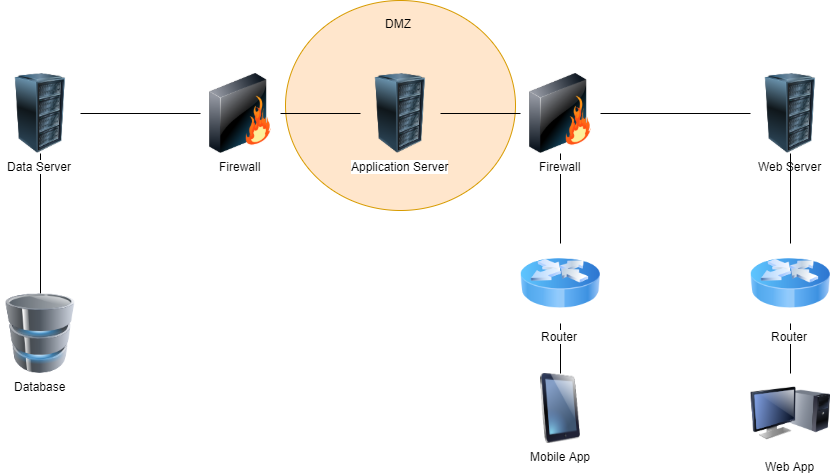
\includegraphics[width=\textwidth,height=\textheight,keepaspectratio]{architecture.png}
\end{figure}
\maketitle

\tableofcontents
\newpage

\section{Document Structure}
\begin{enumerate}

\item \texttt{Introduction}: This section introduces the Design Document. It explains the Purpose, the Scope and the conventions of the document.
\item \texttt{Architectural Design}: This section describes the components used for the system and the relations between them, providing information about their deployment and how they works. It also specifies the architectural styles and the design patterns chosen to design the system.
\item \texttt{User Interface Design}: This section provides an overview on how the User Interface will look like. This section will be accurate enough to explain all our decisions about the design and the UI of the Mobile Application. 
\item \texttt{Implementation, Integration and Testing}: This section contains the order of the system's subcomponents implementation, integration and testing.

\end{enumerate}

\section{Introduction}

\subsection{Purpose}
This document represents the Design Document (DD) for SmartParking mobile application. The purpose of this document is to provide an overall guidance to the architecture of the software product and the interaction between all the components of the system to be developed, following the requirements and the goals that the software must satisfy.

\subsection{Scope}
SmartParking is a crowd-sourced application where users can view all the street parkings around them, together with detailed information. Users can also filter the parkings in several ways: searching for a specific address, a specific type, a maximum distance, etc... Moreover, users can pay the fee directly from the app, chosing the payment type and how much they want to stop.

\subsection{Definition, Acronyms, Abbreviations}

\subsubsection{Definitions}
\begin{itemize}
\item \texttt{User}: any client of the service, a person that logs in the system and uses it.
\item \texttt{User Device}: any compatible device with the SmartParking application, mainly smartphones.
\item \texttt{App}: abbreviation for the SmartParking Mobile Application.
\end{itemize}

\subsubsection{Acronyms}
\begin{itemize}
\item DD: Design Document.
\item API: Application Programming Interface.
\item GPS: Global Positioning System.
\end{itemize}


\subsection{Revision History}
\begin{itemize}
\item 3/04/2020: First Version of DD Document.
\end{itemize}

\subsection{Reference Documents and Used Tools}
\paragraph{Reference Documents}


\paragraph{Used Tools}
\begin{itemize}
\item \textit{Github}: https://github.com/
\item \textit{TexMaker}: https://www.xm1math.net/texmaker/
\item \textit{Draw.io}: https://www.draw.io/
\item \textit{AdobeXD}: https://www.adobe.com/it/products/adobexd.html
\item \textit{LucidChart}: https://www.lucidchart.com/
\end{itemize}


\section{Architectural Design}
Our application is composed by two main components: a Front End, developed with the React Native framework, and a Back End that relies on Firebase, and in particular on Firebase Realtime Database.\\
These two components are highly connected: in fact, the mobile application has the role to show to the user all the data stored in the Database, and also to respond to the user's behaviour.\\
We can say that the mobile App represents the View of the system (in a Model-View-Controller like architecture), the Database represents the Model, and the entire Back End represent the Controller. That is, the App just shows the relevant data to the user, and provide the possibility to choose between some options to modify the shown data.

HIGH LEVEL DIAGRAM - app e db

\subsection{Front End: Mobile Application}
The Mobile Application is a React Native application composed by several screens, each one will be described in the User Interface Design Section. The choiche of React Native frameworks comes from the fact that, being SmartParking an application that will be mainly used "in real time", smartphones will be the target devices: it's more reasonable that a user is using his smartphone when driving (obviously respecting the street law code) rather than a tablet or a smartwatch. A \textbf{cross-platform} framework has been identified as the smartest choiche in this case, in order to reach the largest number of users.\\
This Application will obviously be a \textbf{multi-thread} application. This because we need to be able to handle all user actions and at the same time to keep the Google Map and the shown parkings updated, without having blocking instructions and so performing all the actions in parallel.  

\subsection{Back End: Firebase}
The Firebase back end is where all the parkings, users and reservations data are stored. The back end is also encharged of authentication and user session management (a well implemented and tested functionality of Firebase). 

\subsection{Third Party interaction}
\begin{itemize}
\item \textit{Google}: Login
\item \textit{Facebook}: Login
\item \textit{Paypal}: Parking payments
\item \textit{Stripe}: Parking payments with credit cards
\item \textit{Redux}: Persistent storage of data
\item \textit{Google Maps APIs}: Directions, Distance matrix, Geocoding
\end{itemize}

\section{User Interface Design}
In this section we will describe, page by page, all the Screens of the Mobile Application and their functionalities, along with the decisions we made to provide a nice and pleasant User Experience.
\subsection{Splash Screen}
\subsection{Intro Screen}
\subsection{Login Screen}
\subsection{Registration Screen}
\subsection{Home-Map Screen}
\subsection{List Screen}
\subsection{Filter Screen}
\subsection{Profile Screen}
\subsection{Vehicle Screen}
\subsection{Payment Screen}

\section{Implementation, Integration and test plan}
We can split this section in three main phases: 
\subsection{Front End implementation}
\subsection{Back End implementation}
\subsection{Front End and Back End integration}


\end{document}
